\begin{frame}{La deuda neta del GNC bajó a 58,6\% del PIB en 2025}
\centering
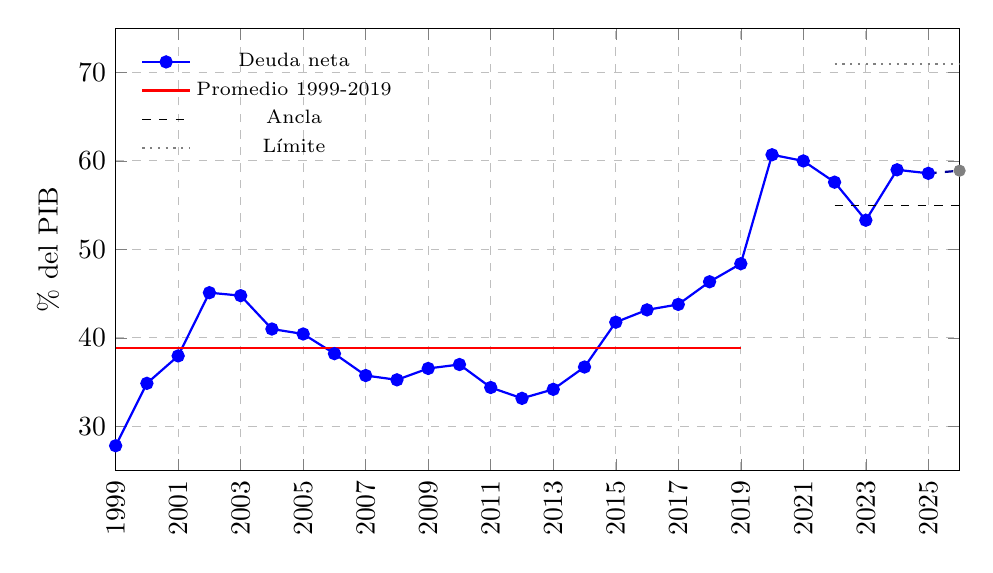
\begin{tikzpicture}
\begin{axis}[
    width=12.3cm,height=7.2cm,
    ylabel={\% del PIB},
    ymin=25,ymax=75,
    xmin=1999,xmax=2026,
    xtick={1999,2001,...,2026},
    xticklabel style={rotate=90,anchor=east,/pgf/number format/.cd,1000 sep={},fixed,precision=0},
    scaled x ticks=false,
    grid=both,
    grid style=dashed,
    legend style={at={(0.02,0.97)},anchor=north west,font=\scriptsize,fill=none,draw=none}
]
\addplot[thick,blue,mark=*] table [row sep=crcr] {
1999 27.8107 \\
2000 34.8664 \\
2001 37.9629 \\
2002 45.1110 \\
2003 44.7733 \\
2004 41.0041 \\
2005 40.4430 \\
2006 38.2196 \\
2007 35.7472 \\
2008 35.2611 \\
2009 36.5470 \\
2010 36.9931 \\
2011 34.3951 \\
2012 33.1683 \\
2013 34.1876 \\
2014 36.7089 \\
2015 41.7724 \\
2016 43.1670 \\
2017 43.7855 \\
2018 46.3437 \\
2019 48.3849 \\
2020 60.7 \\
2021 60.0 \\
2022 57.6 \\
2023 53.3 \\
2024 59.0 \\
2025 58.6 \\
};
\addlegendentry{Deuda neta}
\addplot[thick,red] coordinates {(1999,38.9) (2019,38.9)};
\addlegendentry{Promedio 1999-2019}
\addplot[dashed,black] coordinates {(2022,55) (2026,55)};
\addlegendentry{Ancla}
\addplot[dotted,thick,gray] coordinates {(2022,71) (2026,71)};
\addlegendentry{Límite}
\addplot[color=blue!60!black,dashed,thick] coordinates {(2025,58.6) (2026,58.9)};
\addplot[color=gray,mark=*,only marks] coordinates {(2026,58.9)};
\end{axis}
\end{tikzpicture}
\scriptsize Línea discontinua final: proyección 2026.
\note{[Sources] MFMP 2026, capítulo 1, gráfico 1.9. Serie 1999-2019: MHCP, como en la versión fuente.}
\end{frame}